\documentclass[tikz,border=12pt]{standalone}
\usepackage[T1]{fontenc}
\usepackage{tgheros}
\usepackage{sfmath}
\usepackage{amsmath}
\usepackage{amssymb}
\usepackage{fontawesome5}
\usepackage{tikz}
\usetikzlibrary{arrows.meta,positioning,shapes.geometric,fit,backgrounds,calc}
\usepackage{xcolor}

\renewcommand{\familydefault}{\sfdefault}

% Academic Semantic Palette
\definecolor{harvardcrimson}{HTML}{A51C30}
\definecolor{ethdarkblue}{HTML}{1F407A}
\definecolor{ethblue}{HTML}{215CAF}
\definecolor{ethpetrol}{HTML}{007A87}
\definecolor{ethbronze}{HTML}{B87333}
\definecolor{ethpurple}{HTML}{5B4B8A}
\definecolor{ethslate}{HTML}{475569}
\definecolor{cardbg}{HTML}{F8FAFC}
\definecolor{cardborder}{HTML}{CBD5E1}

\definecolor{boxbluebg}{HTML}{EFF6FF}
\definecolor{boxblueborder}{HTML}{3B82F6}
\definecolor{boxtealbg}{HTML}{ECFDF5}
\definecolor{boxtealborder}{HTML}{10B981}
\definecolor{boxamberbg}{HTML}{FFFBEB}
\definecolor{boxamberborder}{HTML}{F59E0B}
\definecolor{boxpurplebg}{HTML}{F5F3FF}
\definecolor{boxpurpleborder}{HTML}{8B5CF6}

\begin{document}
\begin{tikzpicture}[
  font=\sffamily,
  >=Stealth,
  card/.style={
    draw=cardborder,
    fill=white,
    rounded corners=5pt,
    line width=0.9pt,
    inner sep=8pt,
    align=center
  },
  framebox/.style={
    draw=ethdarkblue,
    fill=white,
    rounded corners=4pt,
    line width=1.1pt,
    inner sep=6pt,
    align=center,
    text=ethdarkblue
  },
  dynarrow/.style={
    ->,
    line width=1.2pt,
    draw=ethblue
  },
  camarrow/.style={
    ->,
    line width=1.2pt,
    draw=ethbronze,
    dashed
  },
  measarrow/.style={
    ->,
    line width=1.2pt,
    draw=ethpetrol
  },
  compnode/.style={
    draw=cardborder,
    fill=cardbg,
    rounded corners=4pt,
    inner sep=5pt,
    align=center
  }
]

  % Top Banner: Title
  \node[card, draw=ethdarkblue, fill=ethdarkblue!5, text width=7.4in, line width=1.1pt] (title) {
    {\large\bfseries\color{ethdarkblue}\faIcon{project-diagram}\;\; DYNAMIC $SE(3)$ COORDINATE FRAME TREE \& TIME-INDEXED BUFFER}\\[3pt]
    {\footnotesize Maintaining spatial metric persistence across asynchronous sensors, moving joints, and Lie algebra ($\mathfrak{se}(3)$) tangent-space integration.}
  };

  % --- LEFT REGION: FRAME GRAPH HIERARCHY ---
  \node[card, draw=ethblue, fill=boxbluebg, text width=3.45in, minimum height=4.3in, below=0.3in of title.south west, anchor=north west] (treecard) {
    {\bfseries\color{ethblue}\faIcon{sitemap}\;\; Coordinate Frame Graph ($T_B^A \in SE(3)$)}\\[6pt]

    \begin{minipage}{3.3in}
      \centering
      % Root Frame: World
      \fcolorbox{ethdarkblue}{white}{
        \begin{minipage}{1.7in}
          \centering\scriptsize\bfseries
          \color{ethdarkblue}\faIcon{globe}\;\; \texttt{world} (Root)\\
          {\tiny Origin: $[0, 0, 0]^T \in \mathbb{R}^3$}
        \end{minipage}
      }\\[12pt]
      
      \faIcon{arrow-down}\;\; {\tiny\color{ethslate}$T_{\text{base}}^{\text{world}}$ (Odometry / Fixed)}\\[6pt]

      % Base Frame: robot_base
      \fcolorbox{ethdarkblue}{white}{
        \begin{minipage}{1.7in}
          \centering\scriptsize\bfseries
          \color{ethdarkblue}\faIcon{cube}\;\; \texttt{robot\_base}\\
          {\tiny Kinematic Center}
        \end{minipage}
      }\\[16pt]

      % Split to Camera and End-Effector
      \begin{minipage}{3.2in}
        \centering
        % Left Branch: Camera
        \begin{minipage}{1.5in}
          \centering
          {\tiny\color{ethbronze}\faIcon{eye}\; $T_{\text{cam}}^{\text{base}}$ (Extrinsic)}\\[2pt]
          \faIcon{arrow-down}\\[2pt]
          \fcolorbox{ethbronze}{white}{
            \begin{minipage}{1.35in}
              \centering\scriptsize\bfseries
              \color{ethbronze}\texttt{camera\_optical}\\
              {\tiny Optical Sensor ($30\text{ Hz}$)}
            \end{minipage}
          }\\[8pt]
          {\tiny\color{harvardcrimson}\faIcon{bullseye}\; $T_{\text{target}}^{\text{cam}}$ (Vision Token)}\\[2pt]
          \faIcon{arrow-down}\\[2pt]
          \fcolorbox{harvardcrimson}{white}{
            \begin{minipage}{1.35in}
              \centering\scriptsize\bfseries
              \color{harvardcrimson}\texttt{target\_object}\\
              {\tiny Target Pose in 3D Space}
            \end{minipage}
          }
        \end{minipage}
        \hfill
        % Right Branch: End-Effector
        \begin{minipage}{1.5in}
          \centering
          {\tiny\color{ethpetrol}\faIcon{cogs}\; $T_{\text{EE}}^{\text{base}}(q)$ ($1\text{ kHz}$ FK)}\\[2pt]
          \faIcon{arrow-down}\\[2pt]
          \fcolorbox{ethpetrol}{white}{
            \begin{minipage}{1.35in}
              \centering\scriptsize\bfseries
              \color{ethpetrol}\texttt{end\_effector}\\
              {\tiny Wrist Link Pose}
            \end{minipage}
          }\\[8pt]
          {\tiny\color{ethdarkblue}\faIcon{hand-paper}\; $T_{\text{tool}}^{\text{EE}}$ (Tool Offset)}\\[2pt]
          \faIcon{arrow-down}\\[2pt]
          \fcolorbox{ethdarkblue}{white}{
            \begin{minipage}{1.35in}
              \centering\scriptsize\bfseries
              \color{ethdarkblue}\texttt{tool\_tip}\\
              {\tiny Grasp Control Point}
            \end{minipage}
          }
        \end{minipage}
      \end{minipage}
    \end{minipage}
  };

  % --- RIGHT REGION: TEMPORAL BUFFER & LIE ALGEBRA INTEGRATION ---
  \node[card, draw=ethpurple, fill=boxpurplebg, text width=3.65in, minimum height=4.3in, right=0.3in of treecard] (buffercard) {
    {\bfseries\color{ethpurple}\faIcon{history}\;\; Time-Indexed Buffer \& Lie Tangent Propagation}\\[6pt]

    \begin{minipage}{3.45in}
      % Step 1: Delayed Observation Arrival
      \fcolorbox{boxamberborder}{white}{
        \begin{minipage}{3.3in}
          \raggedright\scriptsize
          \textbf{\color{ethbronze}\faIcon{stopwatch}\; 1. Delayed Vision Ingestion ($\Delta t_{\text{lag}} = 65\text{ ms}$):}\\
          Vision token arrives at $t_{\text{now}} = 100\text{ ms}$, but photons were transduced at $t_{\text{capture}} = 35\text{ ms}$.\\
          Query buffer for historical transform: $T_{\text{cam}}^{\text{base}}(t=35\text{ ms})$.
        \end{minipage}
      }\\[8pt]

      % Step 2: Coordinate Chaining
      \fcolorbox{boxtealborder}{white}{
        \begin{minipage}{3.3in}
          \raggedright\scriptsize
          \textbf{\color{ethpetrol}\faIcon{link}\; 2. Forward Coordinate Chaining ($SE(3)$):}\\
          $T_{\text{target}}^{\text{world}}(t_{\text{cap}}) = T_{\text{base}}^{\text{world}} \cdot T_{\text{cam}}^{\text{base}}(t_{\text{cap}}) \cdot T_{\text{target}}^{\text{cam}}(t_{\text{cap}})$\\
          Homogeneous matrix multiplication guarantees geometric consistency.
        \end{minipage}
      }\\[8pt]

      % Step 3: Lie Algebra Tangent Space Integration
      \fcolorbox{boxblueborder}{white}{
        \begin{minipage}{3.3in}
          \raggedright\scriptsize
          \textbf{\color{ethdarkblue}\faIcon{calculator}\; 3. Tangent-Space Propagation ($\mathfrak{se}(3)$):}\\
          Forward-integrate from $t_{\text{capture}}$ to $t_{\text{now}}$ using high-rate IMU / joint velocity twists $\boldsymbol{\xi} = [\mathbf{v}, \boldsymbol{\omega}]^T \in \mathbb{R}^6$:\\[3pt]
          \centering
          $\displaystyle T(t_{\text{now}}) = T(t_{\text{capture}}) \cdot \exp\left(\boldsymbol{\xi}^\wedge \cdot \Delta t_{\text{lag}}\right)$\\[3pt]
          \raggedright
          \textbf{Exponential map via Rodrigues formula} prevents gimbal lock singularities and eliminates control lag staleness.
        \end{minipage}
      }\\[8pt]

      % Step 4: Closed-Form Lie algebra formula
      \fcolorbox{ethpurple!40}{white}{
        \begin{minipage}{3.3in}
          \raggedright\scriptsize
          \textbf{\color{ethpurple}\faIcon{shield-alt}\; 4. Real-Time Query Guarantee:}\\
          Lookups execute in $< 10\,\mu\text{s}$ via lock-free ring buffer on Linux MPU and FreeRTOS MCU, enabling $1000\text{ Hz}$ collision checks.
        \end{minipage}
      }
    \end{minipage}
  };

  % Bottom Synthesis Banner
  \node[card, draw=ethdarkblue, fill=ethdarkblue!5, text width=7.4in, below=0.25in of treecard.south west, anchor=north west] (footer) {
    {\bfseries\color{ethdarkblue}\faIcon{check-double}\;\; THE SE(3) FRAME CONTRACT: SPATIAL PERSISTENCE UNDER DELAY}\\[2pt]
    {\footnotesize Dynamic transform graphs decouple sensor arrival rates from motor control cadences. Even if vision lags by $65\text{ ms}$, the system reconstructs the exact metric target pose in real time without coordinate drift.}
  };

\end{tikzpicture}
\end{document}
